\documentclass[10pt, title page]{article}\usepackage[]{graphicx}\usepackage[]{color}
%% maxwidth is the original width if it is less than linewidth
%% otherwise use linewidth (to make sure the graphics do not exceed the margin)
\makeatletter
\def\maxwidth{ %
  \ifdim\Gin@nat@width>\linewidth
    \linewidth
  \else
    \Gin@nat@width
  \fi
}
\makeatother

\definecolor{fgcolor}{rgb}{0.345, 0.345, 0.345}
\newcommand{\hlnum}[1]{\textcolor[rgb]{0.686,0.059,0.569}{#1}}%
\newcommand{\hlstr}[1]{\textcolor[rgb]{0.192,0.494,0.8}{#1}}%
\newcommand{\hlcom}[1]{\textcolor[rgb]{0.678,0.584,0.686}{\textit{#1}}}%
\newcommand{\hlopt}[1]{\textcolor[rgb]{0,0,0}{#1}}%
\newcommand{\hlstd}[1]{\textcolor[rgb]{0.345,0.345,0.345}{#1}}%
\newcommand{\hlkwa}[1]{\textcolor[rgb]{0.161,0.373,0.58}{\textbf{#1}}}%
\newcommand{\hlkwb}[1]{\textcolor[rgb]{0.69,0.353,0.396}{#1}}%
\newcommand{\hlkwc}[1]{\textcolor[rgb]{0.333,0.667,0.333}{#1}}%
\newcommand{\hlkwd}[1]{\textcolor[rgb]{0.737,0.353,0.396}{\textbf{#1}}}%
\let\hlipl\hlkwb

\usepackage{framed}
\makeatletter
\newenvironment{kframe}{%
 \def\at@end@of@kframe{}%
 \ifinner\ifhmode%
  \def\at@end@of@kframe{\end{minipage}}%
  \begin{minipage}{\columnwidth}%
 \fi\fi%
 \def\FrameCommand##1{\hskip\@totalleftmargin \hskip-\fboxsep
 \colorbox{shadecolor}{##1}\hskip-\fboxsep
     % There is no \\@totalrightmargin, so:
     \hskip-\linewidth \hskip-\@totalleftmargin \hskip\columnwidth}%
 \MakeFramed {\advance\hsize-\width
   \@totalleftmargin\z@ \linewidth\hsize
   \@setminipage}}%
 {\par\unskip\endMakeFramed%
 \at@end@of@kframe}
\makeatother

\definecolor{shadecolor}{rgb}{.97, .97, .97}
\definecolor{messagecolor}{rgb}{0, 0, 0}
\definecolor{warningcolor}{rgb}{1, 0, 1}
\definecolor{errorcolor}{rgb}{1, 0, 0}
\newenvironment{knitrout}{}{} % an empty environment to be redefined in TeX

\usepackage{alltt}

%%%%%%%%%%%%%%%%%%%%%%%%%%%%%%%%%%%%%%%%%%%%%%%%%%%%%%%%%%%%
  %%%%%%%%%% load packages                          %%%%%%%%%%
  %%%%%%%%%%%%%%%%%%%%%%%%%%%%%%%%%%%%%%%%%%%%%%%%%%%%%%%%%%%%
  \usepackage{rotating, graphicx, overpic, wrapfig, psfrag, amsfonts, 
    amsmath, amssymb, amsthm, color, fullpage, url, natbib, caption, 
    subcaption, authblk, color, hyperref, bm, blkarray, array, fullpage,
    latexsym, booktabs, enumerate, setspace, enumitem}
\usepackage[boxed]{algorithm2e}

  %%%%%%%%%%%%%%%%%%%%%%%%%%%%%%%%%%%%%%%%%%%%%%%%%%%%%%%%%%%%
  %%%%%%%%%% include macros and set colors          %%%%%%%%%%
  %%%%%%%%%%%%%%%%%%%%%%%%%%%%%%%%%%%%%%%%%%%%%%%%%%%%%%%%%%%%
  \input{macros}


\title{\LARGE {Binormal Example 2} \\ \vspace{.5 cm} {Parametric, Beta, Semiparametric} }
\author{Sarah Stanley}
\date{\today}
\IfFileExists{upquote.sty}{\usepackage{upquote}}{}
\begin{document}

\section{Binormal Example 2}
Data simulated from $Y_D = 2 + 4X + \epsilon_D$ and $Y_{\bar{D}} = 1.5 + 3X + \epsilon_{\bar{D}},$ where $X \sim U(0,1)$ and $\epsilon_D, \epsilon_{\bar{D}} \sim N(0,1.5^2).$  In the following, we include the resulting ROC curves from each of the Parametric, Beta, and Semiparametric methods for specified values of the covariate X as well as the corresponding AUCs.
\subsection{Parametric Method}



\begin{knitrout}
\definecolor{shadecolor}{rgb}{0.969, 0.969, 0.969}\color{fgcolor}\begin{kframe}


{\ttfamily\noindent\bfseries\color{errorcolor}{\#\# Error in setwd("{}C:/Users/Sarah/Desktop/Box Sync/Box Sync"{}): cannot change working directory}}

{\ttfamily\noindent\bfseries\color{errorcolor}{\#\# Error in library(ROCRegression): there is no package called 'ROCRegression'}}\end{kframe}
\end{knitrout}

\begin{knitrout}
\definecolor{shadecolor}{rgb}{0.969, 0.969, 0.969}\color{fgcolor}\begin{kframe}
\begin{alltt}
\hlcom{############ output for alonzo}
\hlkwd{ggplot}\hlstd{(dfParamP,} \hlkwd{aes}\hlstd{(s, ROC))} \hlopt{+} \hlkwd{geom_line}\hlstd{()} \hlopt{+} \hlkwd{facet_grid}\hlstd{(.}\hlopt{~}\hlstd{x)} \hlopt{+} \hlkwd{theme_bw}\hlstd{()} \hlopt{+}
  \hlkwd{labs}\hlstd{(}\hlkwc{title} \hlstd{=} \hlstr{"Parametric ROC for Specified Covariate Values"}\hlstd{)} \hlopt{+}
  \hlkwd{theme}\hlstd{(}\hlkwc{axis.text}\hlstd{=}\hlkwd{element_text}\hlstd{(}\hlkwc{size}\hlstd{=}\hlnum{8}\hlstd{),}
        \hlkwc{panel.margin} \hlstd{=} \hlkwd{unit}\hlstd{(}\hlnum{1}\hlstd{,} \hlstr{"lines"}\hlstd{),} \hlkwc{plot.title} \hlstd{=} \hlkwd{element_text}\hlstd{(}\hlkwc{size}\hlstd{=}\hlnum{12}\hlstd{))} \hlopt{+}
  \hlkwd{scale_x_continuous}\hlstd{(}\hlkwc{name}\hlstd{=}\hlstr{"t"}\hlstd{,} \hlkwc{breaks}\hlstd{=}\hlkwd{seq}\hlstd{(}\hlnum{0}\hlstd{,}\hlnum{1}\hlstd{,}\hlnum{.5}\hlstd{))}
\end{alltt}
\end{kframe}
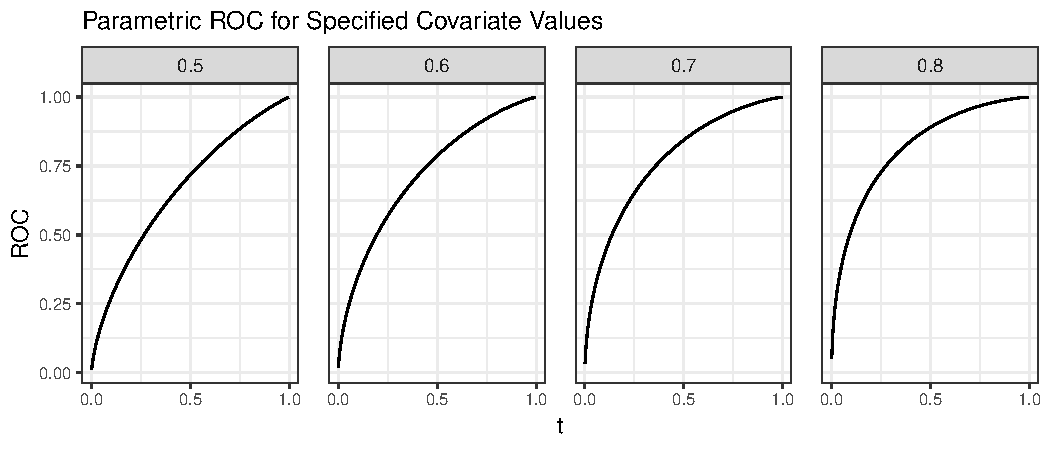
\includegraphics[width=\maxwidth]{figure/unnamed-chunk-2-1} 
\begin{kframe}\begin{alltt}
\hlkwd{round}\hlstd{(aucVecAP2,}\hlnum{4}\hlstd{)}
\end{alltt}
\begin{verbatim}
## [1] 0.6605 0.7164 0.7674 0.8127
\end{verbatim}
\begin{alltt}
\hlkwd{summary}\hlstd{(probitMod)}\hlopt{$}\hlstd{coefficients}
\end{alltt}
\begin{verbatim}
##               Estimate Std. Error   z value     Pr(>|z|)
## (Intercept) -0.5069567 0.02893779 -17.51884 1.028953e-68
## phiInv       0.9239606 0.02001170  46.17101 0.000000e+00
## x            2.1703373 0.05784119  37.52235 0.000000e+00
\end{verbatim}
\end{kframe}
\end{knitrout}

\newpage
%%%%%%%%%%%%%%%%%%%%%%%%%%%%%%%%%%%%%%%%%%%%%%%%%%%%
\subsection{Beta Method}
%%%%%%%%%%%%%%%%%%%%%%%%%%%%%%%%%%%%%%%%%%%%%%%%%%%%



\begin{knitrout}
\definecolor{shadecolor}{rgb}{0.969, 0.969, 0.969}\color{fgcolor}\begin{kframe}


{\ttfamily\noindent\color{warningcolor}{\#\# Warning: `panel.margin` is deprecated. Please use `panel.spacing` property instead}}\end{kframe}
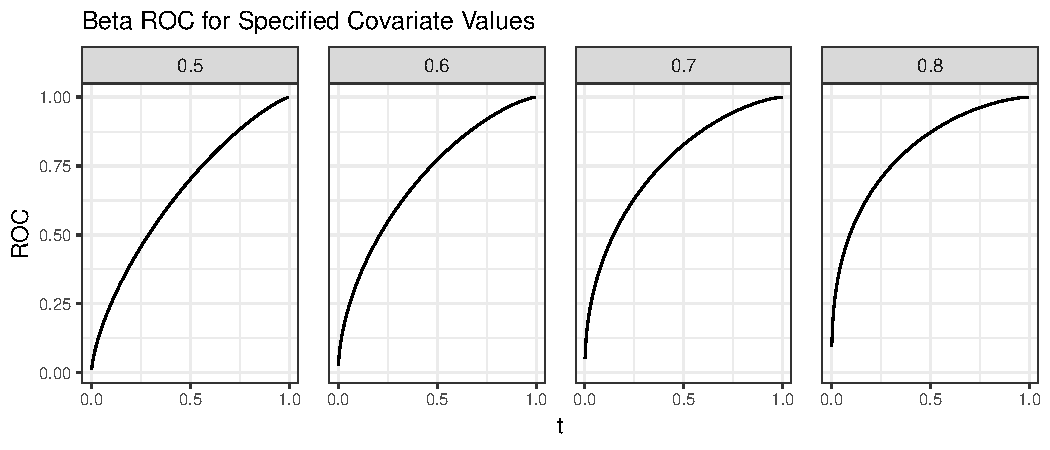
\includegraphics[width=\maxwidth]{figure/unnamed-chunk-4-1} 
\begin{kframe}\begin{verbatim}
## [1] 0.6485 0.7064 0.7581 0.8031
## $mean
##              Estimate Std. Error   z value     Pr(>|z|)
## (Intercept)  0.706540  0.2182316  3.237569 1.205527e-03
## x           -2.673253  0.3983326 -6.711108 1.931516e-11
## 
## $precision
##       Estimate Std. Error  z value     Pr(>|z|)
## (phi) 1.922075  0.2473206 7.771593 7.750529e-15
\end{verbatim}
\end{kframe}
\end{knitrout}


\newpage
%%%%%%%%%%%%%%%%%%%%%%%%%%%%%%%%%%%%%%%%%%%%%%%%%%%%%%%
\subsection{Semiparametric Method}
%%%%%%%%%%%%%%%%%%%%%%%%%%%%%%%%%%%%%%%%%%%%%%%%%%%%%%%



\begin{knitrout}
\definecolor{shadecolor}{rgb}{0.969, 0.969, 0.969}\color{fgcolor}\begin{kframe}
\begin{alltt}
\hlcom{# calculating AUC for specified values of covariate X}
\hlstd{aucVecSemi2} \hlkwb{<-} \hlkwd{sapply}\hlstd{(covVec,} \hlkwa{function}\hlstd{(}\hlkwc{x}\hlstd{)} \hlkwd{auc}\hlstd{(ROCdata, x))}


\hlstd{truth} \hlkwb{<-} \hlkwd{sapply}\hlstd{(covVec,} \hlkwa{function}\hlstd{(}\hlkwc{x}\hlstd{)} \hlkwd{pnorm}\hlstd{((}\hlnum{.5} \hlopt{+} \hlstd{x)}\hlopt{/}\hlkwd{sqrt}\hlstd{(}\hlnum{4.5}\hlstd{)))}

\hlstd{results} \hlkwb{<-} \hlkwd{data.frame}\hlstd{(}\hlstr{"Truth"} \hlstd{= truth,} \hlstr{"Parametric"} \hlstd{= aucVecAP2,} \hlstr{"Semiparametric"} \hlstd{= aucVecSemi2,} \hlstr{"Beta"} \hlstd{= aucVecBeta2)}



\hlstd{label_names} \hlkwb{<-} \hlstd{(}\hlkwd{c}\hlstd{(}\hlstr{'1'} \hlstd{=} \hlstr{"0.5"}\hlstd{,} \hlstr{'2'} \hlstd{=} \hlstr{"0.6"}\hlstd{,} \hlstr{'3'} \hlstd{=} \hlstr{"0.7"}\hlstd{,} \hlstr{'4'} \hlstd{=} \hlstr{"0.8"}\hlstd{))}
\hlkwd{ggplot}\hlstd{(ROCdata,} \hlkwd{aes}\hlstd{(t, ROC))} \hlopt{+} \hlkwd{geom_line}\hlstd{()} \hlopt{+} \hlkwd{facet_grid}\hlstd{(.}\hlopt{~}\hlstd{factor.x,} \hlkwc{labeller} \hlstd{=} \hlkwd{as_labeller}\hlstd{(label_names))} \hlopt{+} \hlkwd{labs}\hlstd{(}\hlkwc{title} \hlstd{=} \hlstr{"SemiParametric ROC for Specified Covariate Values"}\hlstd{)} \hlopt{+}
 \hlkwd{theme}\hlstd{(}\hlkwc{axis.text}\hlstd{=}\hlkwd{element_text}\hlstd{(}\hlkwc{size}\hlstd{=}\hlnum{8}\hlstd{),} \hlkwc{panel.margin} \hlstd{=} \hlkwd{unit}\hlstd{(}\hlnum{1}\hlstd{,} \hlstr{"lines"}\hlstd{),} \hlkwc{plot.title} \hlstd{=} \hlkwd{element_text}\hlstd{(}\hlkwc{size}\hlstd{=}\hlnum{12}\hlstd{))} \hlopt{+} \hlkwd{scale_x_continuous}\hlstd{(}\hlkwc{name}\hlstd{=}\hlstr{"t"}\hlstd{,} \hlkwc{breaks}\hlstd{=}\hlkwd{seq}\hlstd{(}\hlnum{0}\hlstd{,}\hlnum{1}\hlstd{,}\hlnum{.5}\hlstd{))} \hlopt{+}
  \hlkwd{theme_bw}\hlstd{()}
\end{alltt}


{\ttfamily\noindent\color{warningcolor}{\#\# Warning: `panel.margin` is deprecated. Please use `panel.spacing` property instead}}\end{kframe}
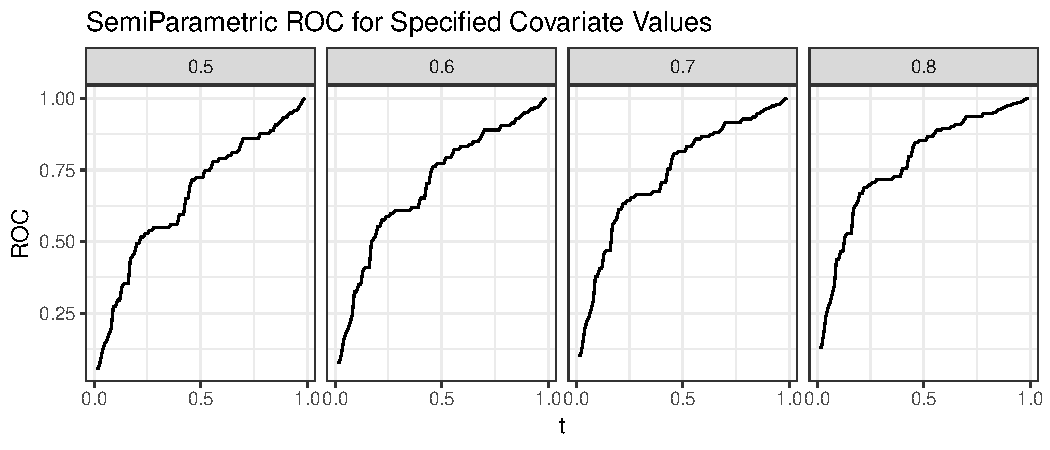
\includegraphics[width=\maxwidth]{figure/unnamed-chunk-6-1} 
\begin{kframe}\begin{alltt}
\hlkwd{round}\hlstd{(aucVecSemi2,}\hlnum{4}\hlstd{)}
\end{alltt}
\begin{verbatim}
## [1] 0.6475 0.6878 0.7256 0.7606
\end{verbatim}
\begin{alltt}
\hlkwd{summary}\hlstd{(probitMod1)}\hlopt{$}\hlstd{coefficients}
\end{alltt}
\begin{verbatim}
##       Estimate Std. Error  z value      Pr(>|z|)
## xDiff 1.496059 0.04978701 30.04918 2.237613e-198
\end{verbatim}
\end{kframe}
\end{knitrout}


\newpage
\subsection{Plot Comparison}



\begin{knitrout}
\definecolor{shadecolor}{rgb}{0.969, 0.969, 0.969}\color{fgcolor}\begin{kframe}
\begin{alltt}
\hlkwd{round}\hlstd{(aucVecAP2,}\hlnum{4}\hlstd{)}
\end{alltt}
\begin{verbatim}
## [1] 0.6605 0.7164 0.7674 0.8127
\end{verbatim}
\begin{alltt}
\hlkwd{round}\hlstd{(aucVecSemi2,} \hlnum{4}\hlstd{)}
\end{alltt}
\begin{verbatim}
## [1] 0.6475 0.6878 0.7256 0.7606
\end{verbatim}
\begin{alltt}
\hlkwd{round}\hlstd{(aucVecBeta2,} \hlnum{4}\hlstd{)}
\end{alltt}
\begin{verbatim}
## [1] 0.6485 0.7064 0.7581 0.8031
\end{verbatim}
\begin{alltt}
\hlkwd{ggplot}\hlstd{(FullPlot2,} \hlkwd{aes}\hlstd{(}\hlkwc{x}\hlstd{=FullPlot2}\hlopt{$}\hlstd{t,} \hlkwc{y}\hlstd{=FullPlot2}\hlopt{$}\hlstd{ROC,} \hlkwc{group}\hlstd{=label))} \hlopt{+}
  \hlkwd{facet_grid}\hlstd{(.}\hlopt{~}\hlstd{x)} \hlopt{+}
 \hlkwd{geom_line}\hlstd{(}\hlkwd{aes}\hlstd{(}\hlkwc{colour} \hlstd{= label),} \hlkwc{lwd} \hlstd{=} \hlnum{1}\hlstd{)} \hlopt{+}
  \hlkwd{theme_bw}\hlstd{()} \hlopt{+} \hlkwd{labs}\hlstd{(}\hlkwc{title} \hlstd{=} \hlstr{"ROC for Specified Covariate Values"}\hlstd{)} \hlopt{+}
  \hlkwd{theme}\hlstd{(}\hlkwc{axis.text}\hlstd{=}\hlkwd{element_text}\hlstd{(}\hlkwc{size}\hlstd{=}\hlnum{15}\hlstd{),} \hlkwc{panel.margin} \hlstd{=} \hlkwd{unit}\hlstd{(}\hlnum{1.5}\hlstd{,} \hlstr{"lines"}\hlstd{),}
        \hlkwc{plot.title} \hlstd{=} \hlkwd{element_text}\hlstd{(}\hlkwc{size}\hlstd{=}\hlnum{14}\hlstd{),}
        \hlkwc{strip.text.x} \hlstd{=} \hlkwd{element_text}\hlstd{(}\hlkwc{size} \hlstd{=} \hlnum{10}\hlstd{),}
        \hlkwc{legend.title}\hlstd{=} \hlkwd{element_text}\hlstd{(}\hlkwc{size} \hlstd{=} \hlnum{10}\hlstd{),}
        \hlkwc{legend.text} \hlstd{=} \hlkwd{element_text}\hlstd{(}\hlkwc{size} \hlstd{=} \hlnum{10}\hlstd{),}
        \hlkwc{text} \hlstd{=} \hlkwd{element_text}\hlstd{(}\hlkwc{size} \hlstd{=} \hlnum{10}\hlstd{))} \hlopt{+}
  \hlkwd{scale_x_continuous}\hlstd{(}\hlkwc{name}\hlstd{=}\hlstr{"t"}\hlstd{,} \hlkwc{breaks}\hlstd{=}\hlkwd{seq}\hlstd{(}\hlnum{0}\hlstd{,}\hlnum{1}\hlstd{,}\hlnum{.5}\hlstd{))} \hlopt{+}
  \hlkwd{scale_y_continuous}\hlstd{(}\hlkwc{name}\hlstd{=}\hlstr{""}\hlstd{)}\hlopt{+}
  \hlkwd{scale_colour_discrete}\hlstd{(}\hlkwc{name} \hlstd{=} \hlstr{"Method"}\hlstd{,} \hlkwc{labels} \hlstd{=} \hlkwd{c}\hlstd{(}\hlstr{"Parametric"}\hlstd{,} \hlstr{"Semiparametric"}\hlstd{,} \hlstr{"Beta"}\hlstd{))}
\end{alltt}


{\ttfamily\noindent\color{warningcolor}{\#\# Warning: `panel.margin` is deprecated. Please use `panel.spacing` property instead}}\end{kframe}
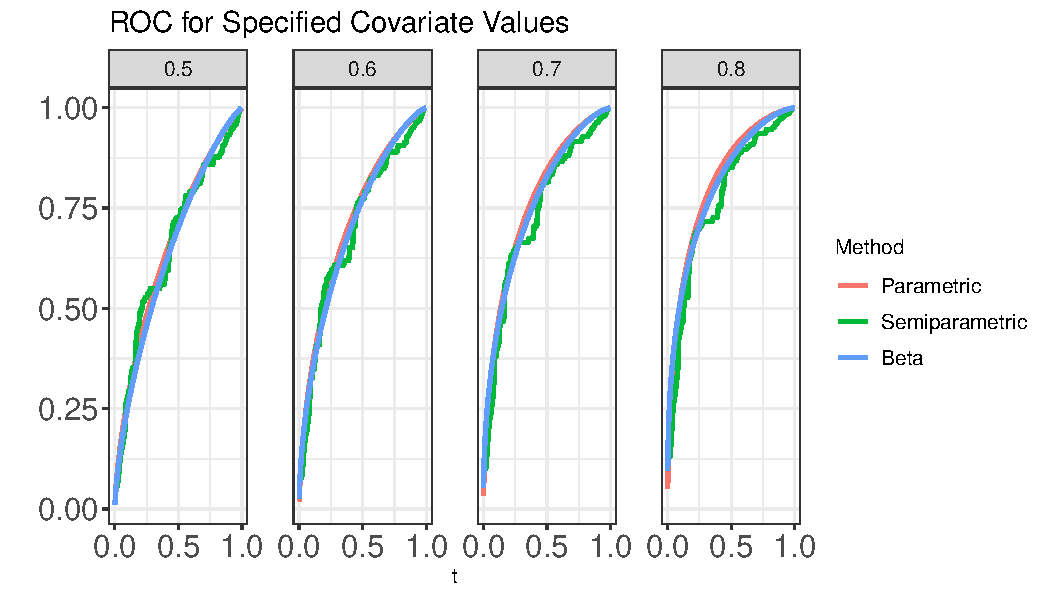
\includegraphics[width=\maxwidth]{figure/unnamed-chunk-8-1} 

\end{knitrout}


\end{document}
